\section{Method}
TriGLE combines representation learning with global and local empirical support for open-set encrypted-traffic recognition. The method characterizes traffic through byte sequences, packet interactions, and multilevel byte organization, and constructs a unified representation through Gaussian adaptation and deterministic fusion. It then combines empirical class centroids with within-class sample neighborhoods to measure deviations from known classes in terms of both global position and local neighborhood relationships. The resulting rejection score integrates global and local information for known-class classification and unknown-class rejection. Fig.~3-1 presents the overall framework.
\begin{figure*}[!t]
\centering
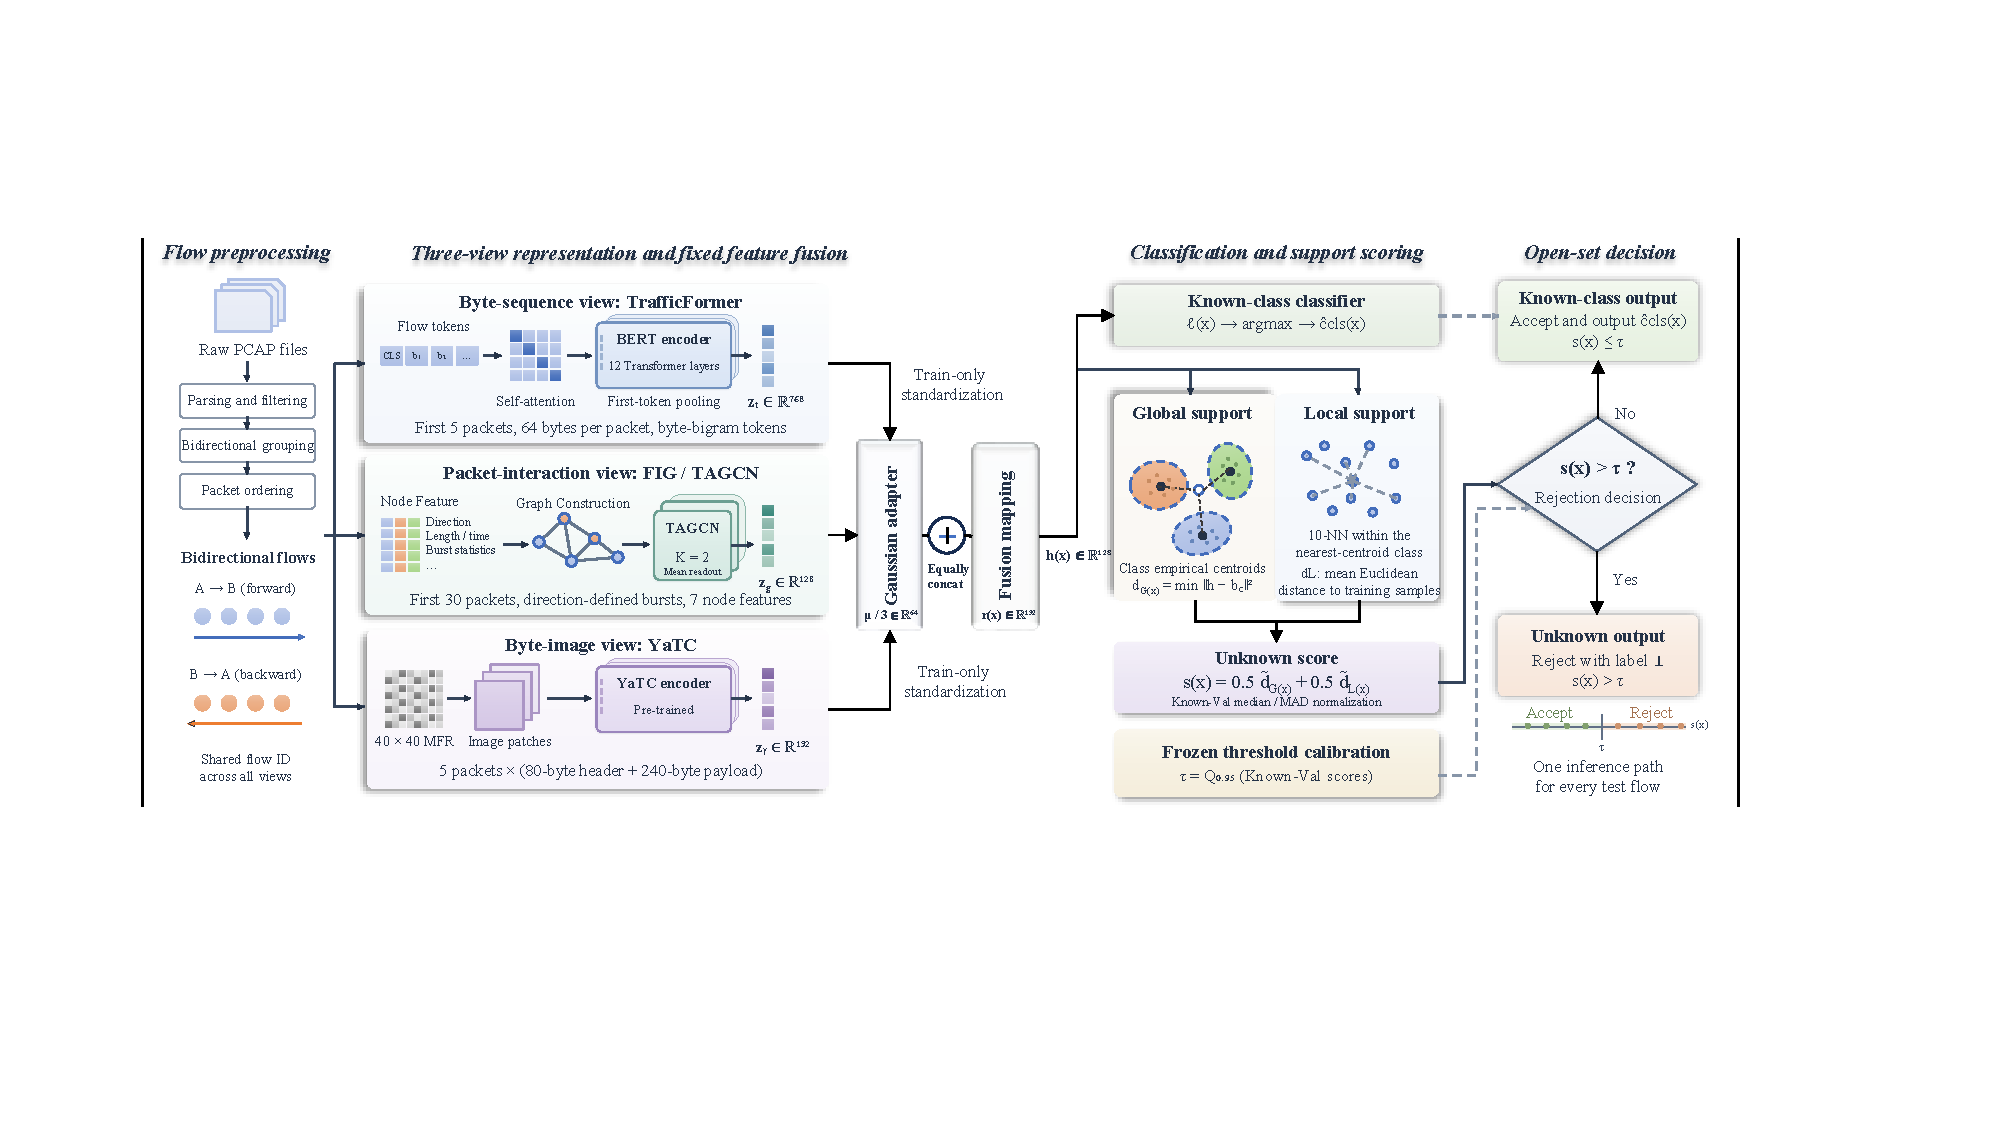
\includegraphics[width=\textwidth,trim=61bp 141bp 119bp 108bp,clip,keepaspectratio]{images/suggestion3_framework.pdf}
\begingroup\renewcommand{\thefigure}{3-1}
\caption{Overall framework of the proposed method.}
\label{fig:framework}\endgroup
\end{figure*}

\subsection{Problem Definition and Notation}
In open-set encrypted-traffic recognition, the labeled training set contains $N$ samples, $\mathcal{D}_{\mathrm{tr}}=\{(x_i,y_i)\}_{i=1}^{N}$. Here, $x_i\in\mathcal{X}$ denotes a bidirectional flow, $\mathcal{X}$ is the traffic sample space, and $y_i\in\mathcal{C}_K=\{1,\ldots,C\}$ is its class label, with $C$ known classes. The known-class validation set is $\mathcal{D}_{\mathrm{val}}$, whose labels also belong to $\mathcal{C}_K$.

At test time, the model processes traffic from both the known-class set $\mathcal{C}_K$ and the unknown-class set $\mathcal{C}_U$. Unknown classes appear in neither the training set nor the validation set, and $\mathcal{C}_K\cap\mathcal{C}_U=\varnothing$. Test samples therefore extend beyond the classes observed during training.

Our objective is to learn an open-set recognition model $f$ that maps an input flow to a known-class label or a unified unknown label:
\begin{equation}
f:\mathcal{X}\rightarrow\mathcal{C}_K\cup\{\bot\},
\tag{1}
\end{equation}
Here, $\bot$ denotes the unknown label. The learning objective has two parts: (1) accurately distinguish flows in $\mathcal{C}_K$ and output their known-class labels; and (2) identify flows in $\mathcal{C}_U$ and assign them the unified unknown label. The model thus addresses both known-class classification and unknown-class rejection. Table~3-1 summarizes the main notation; other symbols are defined at first use.

\begin{table}[!t]\centering\begingroup
\renewcommand{\thetable}{3-1}
\caption{Main notation and definitions}\label{tab:notation}
\fontsize{8}{9.5}\selectfont\setlength{\tabcolsep}{3pt}
\begin{tabular}{@{}p{.31\columnwidth}p{.64\columnwidth}@{}}\hline
Symbol & Definition \\\hline
$\mathcal C_K,\mathcal C_U$ & Known- and unknown-class sets \\
$\mathcal D_{\mathrm{tr}},\mathcal D_{\mathrm{val}}$ & Known training and validation sets \\
$z_v(x),\mu_v(x)$ & Encoded view features and latent mean after Gaussian adaptation \\
$h(x),\ell(x)$ & Fused features and known-class classification score vector \\
$\mathcal T_c,b_c$ & Training representation set and empirical centroid of class $c$ \\
$c^*(x)$ & Class of the nearest centroid \\
$d_G(x),d_L(x)$ & Global centroid distance and local nearest-neighbor distance \\
$s(x),\tau$ & Combined rejection score and rejection threshold \\\hline
\end{tabular}\endgroup\end{table}

\subsection{Traffic Representation Learning in TriGLE}
Encrypted-traffic class characteristics appear in byte combinations and contextual relationships, interactions between packets, and the internal hierarchical structure of packets. We construct byte-sequence, flow-interaction-graph, and byte-image views to learn byte-context dependencies, packet interactions, and multilevel byte organization, respectively. Let $x=\{p_1,p_2,\ldots,p_{n_x}\}$ denote the chronologically ordered packet sequence of a bidirectional flow, where $n_x$ is the packet count. The sending direction of the first packet defines the forward direction. Each branch constructs its input from the same flow and extracts complementary flow-level features for subsequent Gaussian adaptation and fusion.

\subsubsection{Byte-Sequence Branch}
The byte-sequence branch captures local byte-combination patterns and contextual dependencies along the packet-byte sequence. We use pretrained TrafficFormer~\cite{ch2-2} as the byte-sequence encoder to map raw packet bytes to a flow-level sequence representation.

For the chronologically ordered flow $x=\{p_1,p_2,\ldots,p_{n_x}\}$, we select the first $\min(5,n_x)$ packets. After removing the Ethernet header, we retain at most 64 bytes per packet and form hexadecimal byte bigrams following the TrafficFormer input representation. For a byte sequence $(b_1,b_2,\ldots,b_m)$, the bigram representation is $(b_1\Vert b_2,b_2\Vert b_3,\ldots,b_{m-1}\Vert b_m)$, where $\Vert$ denotes concatenation of adjacent bytes. TrafficFormer's token mapping converts these combinations into discrete tokens, which form a flow-level sequence in the original packet order. After adding the $[\mathrm{CLS}]$ token, we truncate or pad the input to a maximum of 320 tokens.

Let $T(x)$ denote the resulting token sequence. We extract features using the pretrained TrafficFormer encoder and fine-tune it with supervision on the known-class training set. The hidden representation at the $[\mathrm{CLS}]$ position in the final encoder layer serves as the flow-level byte-sequence feature:
\begin{equation}
z_t(x)=E_{\mathrm{TF}}\!\left(T(x)\right)_{\mathrm{CLS}}
\in\mathbb{R}^{768},
\tag{2}
\end{equation}
Here, $E_{\mathrm{TF}}$ is the fine-tuned TrafficFormer encoder, and $z_t(x)$ is the 768-dimensional byte-sequence representation used by the subsequent multiview adaptation and fusion module.

\subsubsection{Flow-Interaction-Graph Branch}
The flow-interaction-graph branch characterizes communication behavior through relationships between packets, complementing the low-level content features of the byte-sequence branch. Following existing Flow Interaction Graph (FIG) modeling approaches~\cite{ch2-10,ch2-5}, we represent a bidirectional flow as a packet-level graph. A Topology Adaptive Graph Convolutional Network (TAGCN) learns a structured interaction representation that captures transmission direction, timing, and interaction topology.

For the chronologically ordered flow $x=\{p_1,p_2,\ldots,p_{n_x}\}$, we construct a graph from the first $\min(30,n_x)$ packets, with one node per packet. Consecutive packets with the same sending direction form a burst. Within each burst, edges connect consecutive packets in temporal order. Between adjacent bursts, edges connect their first nodes and their last nodes, capturing transmission continuity and direction changes. This procedure produces an undirected flow interaction graph $G(x)=(V,E)$, where $V$ and $E$ denote the node and edge sets. Fig.~3-2 illustrates burst segmentation, graph construction, node features, and neighborhood aggregation.

\begin{figure}[H]\centering
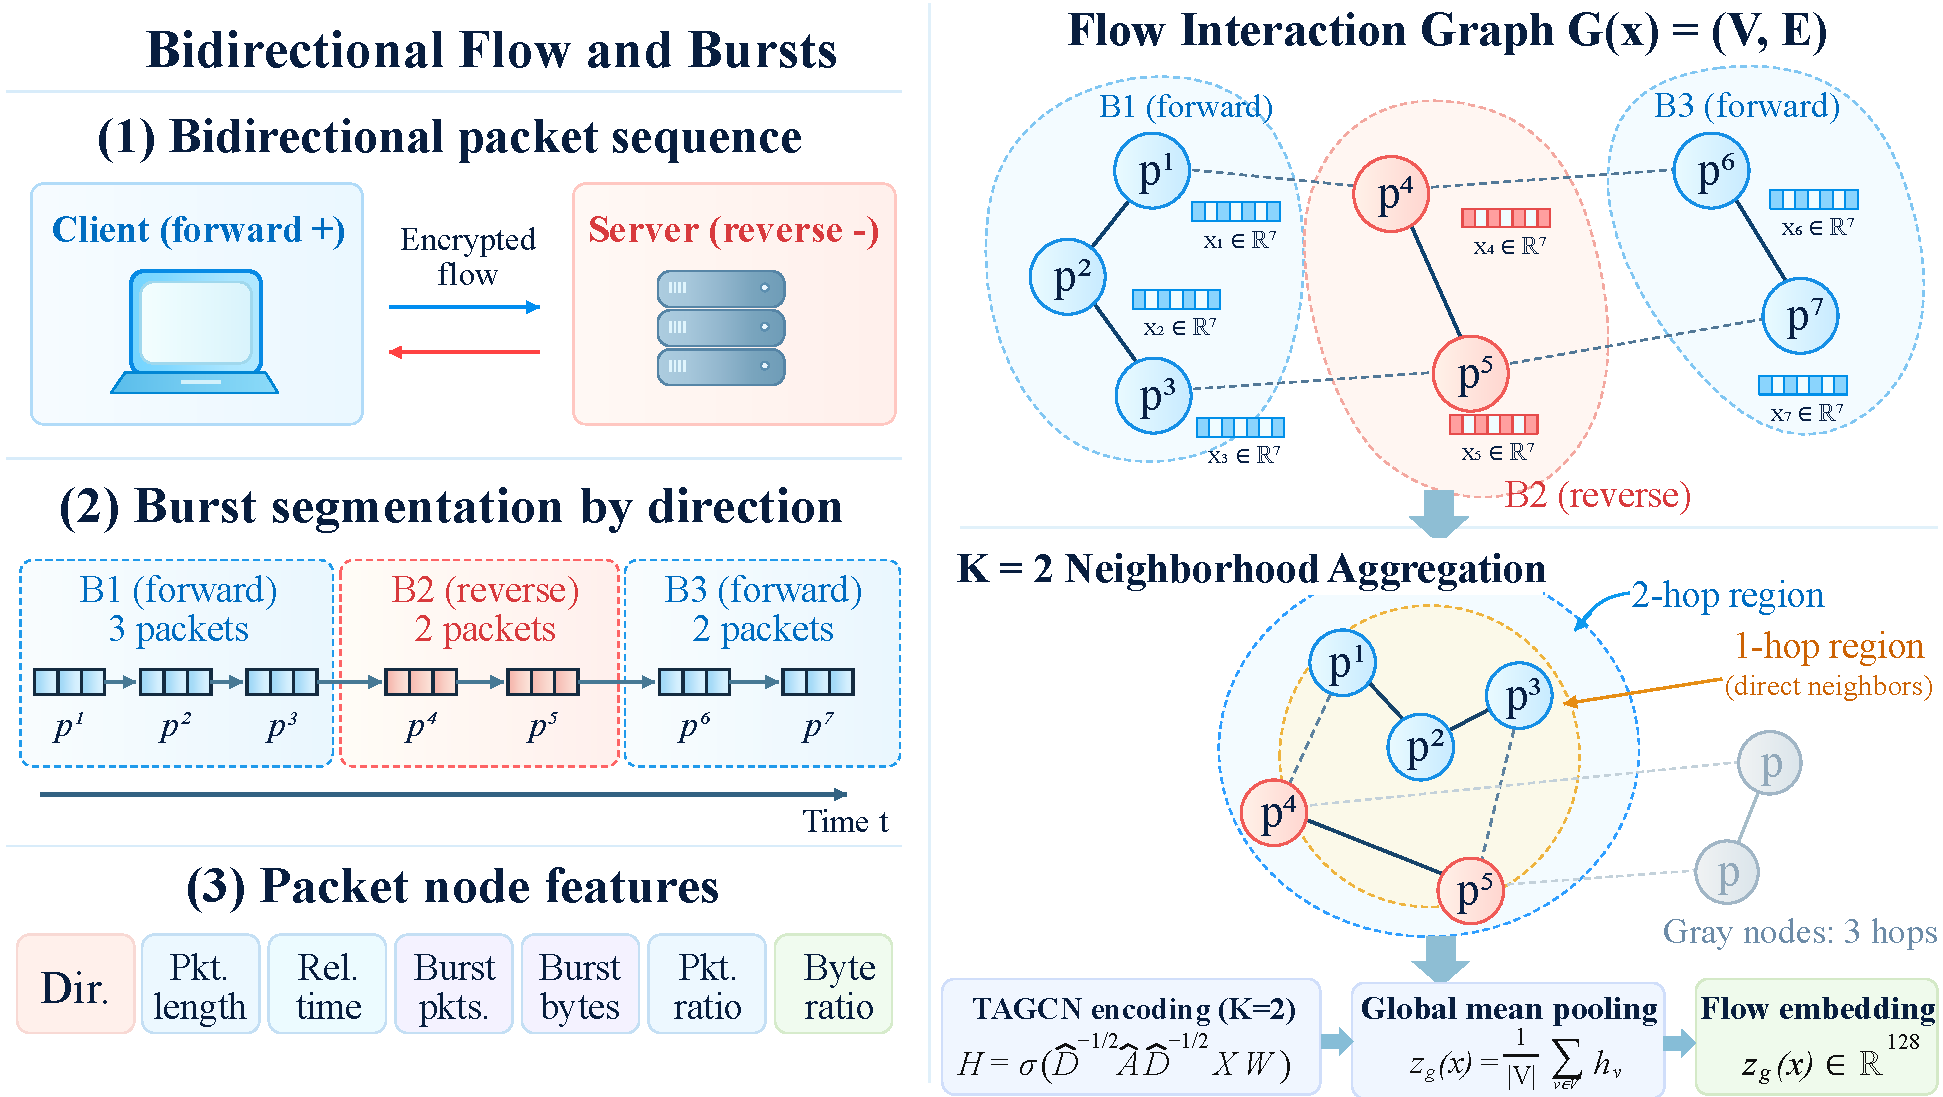
\includegraphics[width=\columnwidth,keepaspectratio]{images/flow-interaction-graph.pdf}
\begingroup\renewcommand{\thefigure}{3-2}
\caption{Flow interaction graph construction and neighborhood aggregation.}
\label{fig:flow-graph}\endgroup\end{figure}

Each node has seven interaction features: sending direction, packet length, elapsed time relative to the first packet, the packet count and total byte count of its burst, and the ratios of the current burst's packet and byte counts to those of the preceding burst. These features describe transmission attributes, local interaction scale, and changes between transmission stages. We collect packet nodes from flows in the known-class training set and compute the mean and standard deviation of each feature dimension. Dimension-wise standardization yields the node-feature matrix $X\in\mathbb{R}^{|V|\times7}$. Validation and testing reuse the training statistics.

TAGCN aggregates neighborhoods of multiple orders to learn structural dependencies between packets. Let $A$ denote the adjacency matrix, with normalized form $\hat{A}=D^{-1/2}(A+I)D^{-1/2}$, where $D$ is the degree matrix of $A+I$. The node-feature update is
\begin{equation}
H=\operatorname{ReLU}\left(
\sum_{k=0}^{2}\hat{A}^{k}XW_k+b
\right),
\tag{3}
\end{equation}
Here, $W_k$ and $b$ are learnable parameters, and $H\in\mathbb{R}^{|V|\times128}$ combines node attributes and multihop topology. Global mean pooling then produces the flow-level graph feature:
\begin{equation}
z_g(x)=\frac{1}{|V|}\sum_{u\in V}H[u,:]
\in\mathbb{R}^{128},
\tag{4}
\end{equation}
The resulting 128-dimensional representation $z_g(x)$ serves as input to multiview adaptation and fusion.

\subsubsection{Byte-Image Branch}
Packet headers and payloads exhibit hierarchical byte organization beyond byte-sequence patterns and packet interactions. Direct concatenation of raw bytes can allocate excessive representation space to longer packets and discard structural information from other packets. Following YaTC's Multi-Level Flow Representation (MFR)~\cite{ch2-4}, we organize raw bytes into a two-dimensional matrix with a fixed layout. Hierarchical encoding captures byte-, packet-, and flow-level structure.

For a bidirectional flow $x$, we select the first five packets and retain an 80-byte header region and a 240-byte payload region per packet, padding missing content with zeros. The fixed header and payload positions form an $8\times40$ packet-level matrix. Stacking these matrices in chronological order yields the $40\times40$ flow-level MFR matrix:
\begin{equation}
B(x)=\operatorname{Stack}(M_1,M_2,\ldots,M_5)
\in\mathbb{R}^{40\times40},
\tag{5}
\end{equation}
Here, $M_i$ is the two-dimensional byte matrix of packet $i$, containing separate header and payload regions. Fixed spatial positions for bytes at different levels preserve within-packet structure and flow-level organization. We normalize byte values to $[-1,1]$ before encoding.

The pretrained YaTC encoder partitions the MFR matrix into nonoverlapping patches and constructs initial features through linear projection and positional embeddings. Packet-level attention first extracts byte relationships within packets, and row pooling (RP) aggregates them into row-level representations:
\begin{equation}
U_p=E_{\mathrm{PL}}(B(x)),\qquad
U_r=\operatorname{RP}(U_p),
\tag{6}
\end{equation}
Here, $E_{\mathrm{PL}}$ comprises patch embedding and packet-level attention, $U_p$ is the packet-level representation, and $U_r$ is the representation after row pooling.

Flow-level attention then models dependencies across packets, and column pooling (CP) produces the flow-level representation:
\begin{equation}
U_f=E_{\mathrm{FL}}(U_r),\qquad
z_y(x)=\operatorname{CP}(U_f)\in\mathbb{R}^{192},
\tag{7}
\end{equation}
Here, $E_{\mathrm{FL}}$ is the flow-level attention encoder, $U_f$ is its output, and $z_y(x)$ is the final 192-dimensional byte-image feature. We initialize the encoder with pretrained YaTC parameters and fine-tune it with supervision on the known-class training set. The resulting multilevel byte features feed the adaptation and fusion module.

\subsection{Gaussian Adaptation and Deterministic Feature Fusion}
The three views capture byte context, packet interactions, and multilevel byte organization, but their feature dimensions and numerical scales differ. We first standardize each encoded view feature $z_v(x)$ using known-training-set statistics, then map it into a common latent space with a view-specific Gaussian adapter. Let $v\in\{t,g,y\}$ index the byte-sequence, flow-interaction-graph, and byte-image views, respectively. The conditional distribution of each latent representation is
\begin{equation}
q_v(u\mid x)
=
\mathcal{N}
\left(
\mu_v(x),
\operatorname{diag}\left(\exp(a_v(x))\right)
\right),
\tag{8}
\end{equation}
Here, $\mu_v(x)$ and $a_v(x)$ denote the latent mean and log variance, respectively. All views share latent dimension $d_u$.

Gaussian adaptation jointly optimizes class discrimination and latent-distribution constraints. During training, reparameterized sampling from $q_v(u\mid x)$ produces latent representations. Classification cross-entropy preserves information relevant to known classes, while KL divergence from the standard normal distribution regularizes the latent distribution. The adaptation objective is
\begin{equation}
\begin{aligned}
\mathcal{L}_{\mathrm{adapt}}={}&\frac{1}{3M}\sum_{i=1}^{M}\sum_{v\in\{t,g,y\}}\Bigl[\mathcal L^{\mathrm{CE}}_{iv}\\
&+\frac{\beta}{d_u}D_{\mathrm{KL}}\left(q_v(u\mid x_i)\,\|\,\mathcal N(0,I)\right)\Bigr].
\end{aligned}\tag{9}
\end{equation}
Here, $M$ is the batch size. For sample $i$ and view $v$, $\mathcal L^{\mathrm{CE}}_{iv}$ is the classification cross-entropy between the true label and the prediction of a view-specific classifier operating on the reparameterized latent sample. The coefficient $\beta$ controls distribution regularization. The classification term preserves class differences, while the KL term constrains deviations from the standard normal distribution.

To eliminate randomness from latent sampling in distance calculations, we construct a deterministic fused representation from the latent means. We scale all three means by the same coefficient, concatenate them, and apply a learnable mapping to obtain fused features. A classification head outputs known-class scores:
\begin{equation}
\begin{aligned}
r(x)&=
\operatorname{concat}
\left(
\frac{\mu_t(x)}{3},
\frac{\mu_g(x)}{3},
\frac{\mu_y(x)}{3}
\right),\\
h(x)&=F_{\varphi}(r(x))\in\mathbb{R}^{128},\\
\ell(x)&=g_{\psi}(h(x))\in\mathbb{R}^{C}.
\end{aligned}
\tag{10}
\end{equation}
Here, $r(x)$ is the concatenated representation, $F_{\varphi}$ learns combinations of features across views, and $g_{\psi}$ is the known-class classification head. The score $\ell_c(x)$ corresponds to class $c$. Global and local empirical support modeling also uses $h(x)$, placing known-class classification and unknown-class discrimination in the same representation space.

\subsection{Global and Local Empirical Support Modeling}
Known-class classification distinguishes classes, whereas unknown-class discrimination must also assess a test sample's relationship to known training samples. Class centroids summarize the overall location of training representations but cannot fully characterize within-class distributions. A sample near a centroid may still lie far from actual training samples. We therefore combine class centroids and within-class nearest neighbors in the fused space to characterize deviations in global position and local proximity. In the learned, fixed representation space, known training samples define a reference set for each class:
\begin{equation*}
\begin{gathered}
\mathcal{T}_c=\{h(x_i):y_i=c,(x_i,y_i)\in\mathcal{D}_{\mathrm{tr}}\},
\\
N_c=|\mathcal{T}_c|.
\end{gathered}
\end{equation*}
Here, $\mathcal T_c$ is the training representation set of known class $c$, and $N_c$ is its size. The mean representation $b_c$ serves as the empirical centroid, summarizing the class's overall position. For a test flow $x$, distances to all class centroids determine the nearest-centroid class $c^*(x)$. The corresponding squared Euclidean distance defines the global distance $d_G(x)$:
\begin{equation}
\begin{aligned}
b_c&=\frac{1}{N_c}\sum_{h_i\in\mathcal{T}_c}h_i,\\
c^*(x)&=\operatorname*{arg\,min}_{c\in\mathcal{C}_K}
\|h(x)-b_c\|_2^2,\\
d_G(x)&=\|h(x)-b_{c^*(x)}\|_2^2.
\end{aligned}
\tag{11}
\end{equation}
The global distance measures deviation from the nearest class centroid. To characterize proximity to actual training representations, we select the $k$ representations nearest to $h(x)$ in Euclidean distance from $\mathcal{T}_{c^*(x)}$. These representations form the local neighborhood $\mathcal{N}_k(x)$. The local distance is their mean distance to the test representation:
\begin{equation}
d_L(x)=
\frac{1}{k}
\sum_{h_j\in\mathcal{N}_k(x)}
\|h(x)-h_j\|_2,
\qquad
\mathcal{N}_k(x)\subseteq\mathcal{T}_{c^*(x)}.
\tag{12}
\end{equation}
A larger $d_L(x)$ indicates greater separation from the selected class's training neighborhood and thus weaker local empirical support. Global and local distances provide complementary geometric evidence of deviation from the class's overall location and actual training neighborhood. The nearest-centroid class $c^*(x)$ selects the class for neighborhood construction. The classification head still determines the final known-class label of an accepted sample; the two class assignments need not agree.

\subsection{Robust Standardization and Open-Set Decision}
The global distance $d_G(x)$ is a squared Euclidean distance to a centroid, whereas $d_L(x)$ is a mean Euclidean distance to within-class neighbors. Their numerical scales differ, so direct combination can allow one distance to dominate. We robustly standardize them separately using the known-class validation set. For $a\in\{G,L\}$, let $\mathcal{S}_a=\{d_a(x):x\in\mathcal{D}_{\mathrm{val}}\}$. Its median $m_a$ and median absolute deviation $\mathrm{MAD}_a$ describe location and dispersion, yielding
\begin{equation}
\begin{gathered}
m_a=\operatorname{median}(\mathcal{S}_a),\\
\mathrm{MAD}_a=\operatorname{median}_{u\in\mathcal{S}_a}|u-m_a|,
\\
\tilde d_a(x)=\frac{d_a(x)-m_a}{\mathrm{MAD}_a+\varepsilon}.
\end{gathered}\tag{13}
\end{equation}
Here, the positive constant $\varepsilon>0$ prevents division by zero. Fixed equal weights combine the standardized distances into the rejection score $s(x)$. The empirical 95\% quantile of known-validation scores determines the threshold $\tau$:
\begin{equation}
\begin{gathered}
s(x)=\frac{1}{2}\tilde d_G(x)+\frac{1}{2}\tilde d_L(x),
\\
\tau=Q_{0.95}\left(\{s(x):x\in\mathcal{D}_{\mathrm{val}}\}\right).
\end{gathered}\tag{14}
\end{equation}
Here, $Q_{0.95}$ denotes the empirical quantile operator. Both the standardization statistics and the rejection threshold come from the known-class validation set. A higher $s(x)$ indicates greater combined deviation from known-class centroids and training neighborhoods. Scores above the threshold trigger an unknown decision. Otherwise, the classification head predicts $\hat c_{\mathrm{cls}}(x)=\operatorname*{arg\,max}_{c\in\mathcal C_K}\ell_c(x)$. The final open-set decision rule is
\begin{equation}
f(x)=
\begin{cases}
\hat c_{\mathrm{cls}}(x), & s(x)\le\tau,\\
\bot, & s(x)>\tau,
\end{cases}
\tag{15}
\end{equation}
Here, $\bot$ is the unified unknown-class label.
